\documentclass[a4paper,12pt]{article}
\usepackage[utf8]{inputenc}
\usepackage[english]{babel} % For English language and hyphenation
\usepackage{amsmath, amssymb}
\usepackage{graphicx}
\usepackage{hyperref} % For references to external documents
\usepackage{physics} % For enhanced physical notation
\usepackage{siunitx} % For SI units
\usepackage{tikz} % For diagrams
\usepackage{setspace} % For line spacing
\usepackage{tcolorbox} % For highlighted text boxes

\begin{document}
	
	\title{Real Consequences of Reformulating Time and Mass in Physics: Beyond the Planck Scale}
	\author{Johann Pascher}
	\date{March 24, 2025}
	\maketitle
	
	\tableofcontents % Table of contents
	\newpage % Optional: Starts the main body on a new page
	
	\section{Introduction}
	This paper explores the real consequences of reformulating fundamental physical concepts, particularly time and mass, as introduced in my previous studies: \textit{Complementary Extensions of Physics: Absolute Time and Intrinsic Time} (March 24, 2025), \textit{A Model with Absolute Time and Variable Energy: A Detailed Investigation of the Foundations} (March 24, 2025), and \textit{Time as an Emergent Property in Quantum Mechanics} (March 23, 2025). These works propose alternative frameworks—absolute time with variable mass and a mass-dependent intrinsic time—that challenge conventional interpretations of special relativity and quantum mechanics. Before delving into the implications, it is crucial to establish the boundaries within which these models hold: the speed of light (\( c_0 \approx 3 \times 10^8 \, \text{m/s} \)) and the Planck mass (\( m_P = \sqrt{\frac{\hbar c_0}{G}} \approx 2.176 \times 10^{-8} \, \text{kg} \)) define the domains where these approaches apply. Nevertheless, the conceptual models extend beyond these limits, opening a speculative yet physically significant realm between the singularity (Planck scale) and the speed of light, as well as masses smaller than the Planck mass. This document examines the interpretive and practical consequences of these reformulations, emphasizing their potential to transform our understanding of physical reality.
	
	\section{Defining the Boundaries: Speed of Light and Planck Mass}
	The speed of light \( c_0 \) and the Planck mass \( m_P \) serve as fundamental constraints in modern physics, delineating the regions where the proposed models are valid. The speed of light represents the upper velocity limit in both the standard model of special relativity (SRT) and the \( T_0 \)-model with absolute time, ensuring causality and the consistency of spacetime interactions. The Planck mass, derived from fundamental constants (\( \hbar \), \( c_0 \), and the gravitational constant \( G \)), marks the scale where quantum gravitational effects become significant, typically associated with the Planck time (\( t_P = \sqrt{\frac{\hbar G}{c_0^5}} \approx 5.39 \times 10^{-44} \, \text{s} \)) and the Planck length (\( l_P = \sqrt{\frac{\hbar G}{c_0^3}} \approx 1.616 \times 10^{-35} \, \text{m} \)).
	
	\begin{tcolorbox}[colback=blue!5!white,colframe=blue!75!black,title=Model Definitions]
		\textbf{Standard Model of SRT:}
		\begin{itemize}
			\item Time dilation: $t' = \gamma t$
			\item Rest mass constant: $m_0 = \text{const.}$
			\item Relativistic mass: $m_{rel} = \gamma m_0$
			\item Energy: $E = m_{rel}c_0^2$
		\end{itemize}
		
		\textbf{$T_0$-Model with Absolute Time:}
		\begin{itemize}
			\item Time absolute: $T_0 = \text{const.}$
			\item Mass variable: $m = \gamma m_0$
			\item Energy: $E = \frac{\hbar}{T_0}$
		\end{itemize}
		
		\textbf{Modified Schrödinger Equation:}
		\begin{itemize}
			\item Intrinsic time: $T = \frac{\hbar}{mc^2}$
			\item Time evolution: $i\hbar\frac{\partial\psi}{\partial t} = \frac{t}{T}H\psi$
		\end{itemize}
	\end{tcolorbox}
	
	In standard SRT, time dilation (\( t' = \gamma t \)) and a constant rest mass (\( m_0 \)) govern relativistic phenomena, whereas in the \( T_0 \)-model, time remains absolute (\( T_0 \)), and mass varies (\( m = \gamma m_0 \)) with energy defined as (\( E = \frac{\hbar}{T_0} \)). Similarly, the modified Schrödinger equation introduces an intrinsic time (\( T = \frac{\hbar}{m c^2} \)), scaling the system's evolution with mass. These reformulations are mathematically consistent within the boundaries of \( c_0 \) and \( m_P \), as they equivalently reproduce observable phenomena (e.g., GPS corrections, muon decay) to the standard model. However, their conceptual reach extends beyond these limits, exploring regions near singularities and masses below the Planck mass, where traditional interpretations falter.
	
	\section{Beyond the Boundaries}
	Despite the established limits, the proposed models invite exploration beyond \( c_0 \) and \( m_P \), creating a theoretical space between the Planck scale singularity and the speed of light, as well as masses below \( m_P \). This extension arises from the flexibility of the concepts of absolute time (\( T_0 \)) and intrinsic time (\( T \)):
	
	- \textbf{Near the Singularity}: At the Planck scale, where \( t_P \) and \( m_P \) dominate, the standard model predicts a collapse of the classical spacetime continuum due to infinite densities. In contrast, the \( T_0 \)-model posits a constant time, allowing mass and energy to scale (\( m = \frac{\hbar}{T_0 c_0^2} \)) without assuming variable time. This suggests a finite, albeit extreme, energy state rather than a singularity.
	- \textbf{Sub-Planck Masses}: For masses \( m < m_P \), the intrinsic time \( T = \frac{\hbar}{m c^2} \) exceeds \( t_P \), implying slower time evolution for lighter particles. This challenges the notion of a universal minimal timescale and opens possibilities for quantum systems below the Planck threshold.
	- \textbf{Speed of Light}: While \( c_0 \) remains inviolable, the reformulations shift focus from time dilation to mass variation, potentially altering the behavior of systems near this boundary.
	
	\begin{figure}[h]
		\centering
		\begin{tikzpicture}
			\draw[->] (0,0) -- (6,0) node[right] {Mass $m$};
			\draw[->] (0,0) -- (0,4) node[above] {Intrinsic Time $T$};
			\draw[scale=0.5, domain=0.1:10, smooth, variable=\x, blue, thick] plot ({\x}, {1/\x});
			\draw[dotted, red] (1.5,0) -- (1.5,1.5) -- (0,1.5);
			\node at (1.5,-0.3) {$m_P$};
			\node at (-0.3,1.5) {$t_P$};
			\node[blue] at (4.5,2) {$T = \frac{\hbar}{mc^2}$};
		\end{tikzpicture}
		\caption{Relationship between mass and intrinsic time. Below the Planck mass ($m_P$), the intrinsic time ($T$) exceeds the Planck time ($t_P$).}
	\end{figure}
	
	This speculative domain, though not directly testable with current technology, provides a framework to rethink extreme physical conditions.
	
	\section{Real Interpretive Consequences}
	
	\subsection{Cosmological Implications}
	In cosmology, the standard model interprets redshift as evidence of an expanding universe driven by time dilation and fixed rest mass. The \( T_0 \)-model, however, suggests that redshift could result from an energy or mass loss (\( E = m c^2 \)) over constant time, implying a static or differently evolving universe. For instance, the cosmic microwave background (CMB) temperature (\( T = 2.725 \, \text{K} \)) could be viewed as a static field with mass gradients rather than a relic of expansion. This reinterpretation challenges the Big Bang singularity, replacing it with a high-energy, mass-rich state at \( T_0 \), potentially resolving issues like the horizon problem without inflation.
	
	\begin{tcolorbox}[colback=green!5!white,colframe=green!75!black,title=Reinterpretation of Cosmological Phenomena]
		\textbf{Standard Model:}
		\begin{itemize}
			\item Redshift $z = \frac{\lambda_{observed} - \lambda_{emitted}}{\lambda_{emitted}}$ as a result of expansion
			\item CMB as cooled radiation from the early universe
			\item Big Bang as an initial singularity
		\end{itemize}
		
		\textbf{$T_0$-Model:}
		\begin{itemize}
			\item Redshift as energy loss $E_2 = E_1(1+z)^{-1}$
			\item CMB as a static field with mass gradients
			\item High-energy state instead of a singularity
		\end{itemize}
		
		\textbf{Testable Predictions:}
		\begin{itemize}
			\item Deviations in the redshift-distance relationship
			\item CMB anisotropies with mass-dependent characteristics
			\item Altered primordial nucleosynthesis patterns
		\end{itemize}
	\end{tcolorbox}
	
	\subsection{Quantum Mechanics and Gravitation}
	The intrinsic time \( T = \frac{\hbar}{m c^2} \) in the modified Schrödinger equation ties quantum evolution to mass, offering a bridge to quantum gravitation. For masses near or below \( m_P \), where \( T \) exceeds \( t_P \), slower time evolution could stabilize quantum states and enable coherence in extreme gravitational fields (e.g., near black holes). Conversely, the absolute time of the \( T_0 \)-model suggests that gravitational effects might arise from energy gradients (\( E_{grav} = \sqrt{\frac{\hbar E^5}{G}} \)), redefining spacetime curvature as an emergent property of mass variation rather than time distortion.
	
\subsection{Nonlocality in Quantum Physics}
A key feature of quantum physics is nonlocality, observed in entanglement, often interpreted as "instantaneous" correlation across spatial distances. In the standard model, time is relativistically variable, preserving the causal structure of light cones, while nonlocality is explained by correlations without signal transmission. True instantaneity would only occur if the Planck mass were zero, which is physically excluded. The \( T_0 \)-model with absolute time offers an alternative: since \( T_0 \) is constant, entangled states could correlate via mass variation (\( m = \gamma m_0 \)) or energy (\( E = \frac{1}{T_0} \)) without requiring temporal mediation. These correlations would thus not be "instantaneous" but an expression of.mass or energy dynamics.

The modified Schrödinger equation with intrinsic time, in Planck units \( T = \frac{1}{m} \) for massive particles, reinforces this view. As \( T \) is mass-dependent, the states of entangled particles evolve at different rates. A particle with smaller mass (larger \( T \)) exhibits slower time evolution, implying delays in state changes compared to a heavier counterpart (smaller \( T \)). For example, in an entangled electron-muon pair, the correlation might not be instantaneous but exhibit a measurable delay scaling with \( T_e / T_\mu = m_\mu / m_e \). This frames nonlocality as an emergent property of the mass-time relationship, contradicting the assumption of universal simultaneity. Experimentally, this could be tested via Bell tests with particles of different masses, measuring correlation times to detect delays as a function of mass.

\begin{figure}[h]
	\centering
	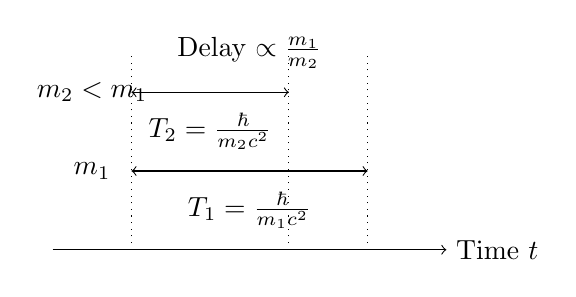
\begin{tikzpicture}
		\draw[->] (0,0) -- (5,0) node[right] {Time $t$};
		\draw[<->] (1,1) -- (4,1);
		\draw[<->] (1,2) -- (3,2);
		\node at (0.5,1) {$m_1$};
		\node at (0.5,2) {$m_2 < m_1$};
		\draw[dotted] (1,0) -- (1,2.5);
		\draw[dotted] (3,0) -- (3,2.5);
		\draw[dotted] (4,0) -- (4,2.5);
		\node at (2.5,0.5) {$T_1 = \frac{\hbar}{m_1c^2}$};
		\node at (2,1.5) {$T_2 = \frac{\hbar}{m_2c^2}$};
		\node at (2.5,2.5) {Delay $\propto \frac{m_1}{m_2}$};
	\end{tikzpicture}
	\caption{Delayed correlation in entangled particles of different masses. The lighter particle ($m_2$) evolves slower than the heavier one ($m_1$).}
\end{figure}

An additional challenge arises with massless particles like photons (\( m = 0 \)), which possess only kinetic energy (\( E = p \)). In the original formulation, \( m = 0 \) yields an infinite \( T = \frac{1}{m} \), halting time evolution and clashing with the standard description. Similarly, in the \( T_0 \)-model, mass variability for photons remains undefined. In Planck units (\( \hbar = c_0 = G = 1 \)), this can be resolved by an extension: \( T = \frac{1}{E} \) for massless particles. For a photon with \( E = p \), this yields \( T = \frac{1}{p} \), corresponding to its wavelength. This simplification eliminates constants, as \( T = \frac{\hbar}{m c^2} \) becomes \( T = \frac{1}{m} \) and \( T = \frac{\hbar}{E} \) becomes \( T = \frac{1}{E} \), with \( E = m \) for massive particles and \( E = p \) for massless ones. In an entangled photon-massive particle system (e.g., photon and electron), the correlation depends on \( T_\text{photon} = \frac{1}{p} \) and \( T_e = \frac{1}{m_e} \), implying distinct delays. A unified time definition \( T = \frac{1}{\max(m, E)} \) enables consistent treatment, where \( m \) dominates for massive particles and \( E \) for massless ones, adjusting the Schrödinger equation to \( i \frac{\partial \psi}{\partial (t/T)} = H \psi \), with \( H = p \) for photons and \( H = -\frac{1}{2m} \nabla^2 + V \) for massive particles. The detailed implications of this extension for photon nonlocality, particularly the shift from instantaneous to energy-dependent correlations, are elaborated in the separate document \textit{Implications of Energy-Dependent Time Definition for Photon Nonlocality}.
	\begin{figure}[h]
		\centering
		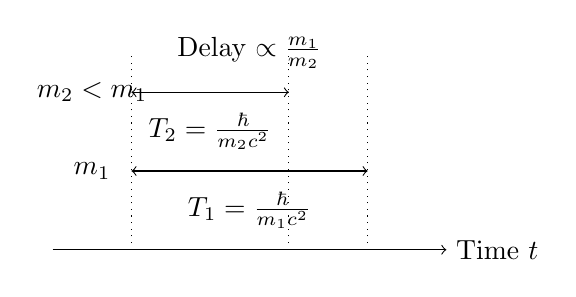
\begin{tikzpicture}
			\draw[->] (0,0) -- (5,0) node[right] {Time $t$};
			\draw[<->] (1,1) -- (4,1);
			\draw[<->] (1,2) -- (3,2);
			\node at (0.5,1) {$m_1$};
			\node at (0.5,2) {$m_2 < m_1$};
			\draw[dotted] (1,0) -- (1,2.5);
			\draw[dotted] (3,0) -- (3,2.5);
			\draw[dotted] (4,0) -- (4,2.5);
			\node at (2.5,0.5) {$T_1 = \frac{\hbar}{m_1c^2}$};
			\node at (2,1.5) {$T_2 = \frac{\hbar}{m_2c^2}$};
			\node at (2.5,2.5) {Delay $\propto \frac{m_1}{m_2}$};
		\end{tikzpicture}
		\caption{Delayed correlation in entangled particles of different masses. The lighter particle ($m_2$) evolves slower than the heavier one ($m_1$).}
	\end{figure}
	
	An additional challenge arises with massless particles like photons (\( m = 0 \)), which possess only kinetic energy (\( E = p \)). In the original formulation, \( m = 0 \) yields an infinite \( T = \frac{1}{m} \), halting time evolution and clashing with the standard description. Similarly, in the \( T_0 \)-model, mass variability for photons remains undefined. In Planck units (\( \hbar = c_0 = G = 1 \)), this can be resolved by an extension: \( T = \frac{1}{E} \) for massless particles. For a photon with \( E = p \), this yields \( T = \frac{1}{p} \), corresponding to its wavelength. This simplification eliminates constants, as \( T = \frac{\hbar}{m c^2} \) becomes \( T = \frac{1}{m} \) and \( T = \frac{\hbar}{E} \) becomes \( T = \frac{1}{E} \), with \( E = m \) for massive particles and \( E = p \) for massless ones. In an entangled photon-massive particle system (e.g., photon and electron), the correlation depends on \( T_\text{photon} = \frac{1}{p} \) and \( T_e = \frac{1}{m_e} \), implying distinct delays. A unified time definition \( T = \frac{1}{\max(m, E)} \) enables consistent treatment, where \( m \) dominates for massive particles and \( E \) for massless ones, adjusting the Schrödinger equation to \( i \frac{\partial \psi}{\partial (t/T)} = H \psi \), with \( H = p \) for photons and \( H = -\frac{1}{2m} \nabla^2 + V \) for massive particles. The detailed implications of this extension for photon nonlocality, particularly the shift from instantaneous to energy-dependent correlations, are elaborated in the separate document \textit{Implications of Energy-Dependent Time Definition for Photon Nonlocality}.
	
	\subsection{Connection to Quantum Field Theory}
	Quantum field theory (QFT) describes particles as field excitations, with time and space as continuous coordinates and rest mass \( m_0 \) invariant. The proposed models directly impact this framework. In the \( T_0 \)-model, time is assumed absolute, and mass varies with energy (\( m = \frac{\hbar}{T_0 c_0^2} \)). This could imply that field excitations are characterized not by a fixed rest mass but by dynamic energy states scaling with \( T_0 \). In QFT, this might necessitate redefining propagators, as the time coordinate no longer varies relativistically, and mass becomes the primary variable. A possible adjustment could be:
	\[
	G(x, T_0) = \int \frac{d^4p}{(2\pi)^4} \frac{e^{-ip \cdot x}}{p^2 - (m(T_0))^2 + i\epsilon},
	\]
	where \( m(T_0) = \frac{\hbar}{T_0 c_0^2} \) is a time-independent but energy-dependent mass.
	
	\begin{tcolorbox}[colback=yellow!5!white,colframe=yellow!75!black,title=Reformulation of QFT Concepts]
		\textbf{Standard QFT:}
		\begin{align}
			S &= \int d^4x \mathcal{L}(\phi, \partial_\mu\phi) \\
			\mathcal{L} &= \frac{1}{2}(\partial_\mu\phi)(\partial^\mu\phi) - \frac{1}{2}m_0^2\phi^2 - V(\phi)
		\end{align}
		
		\textbf{$T_0$-Model in QFT:}
		\begin{align}
			S &= \int d^3x \int dT_0 \mathcal{L}(\phi, \partial_i\phi, \partial_{T_0}\phi) \\
			\mathcal{L} &= \frac{1}{2}(\partial_i\phi)(\partial^i\phi) - \frac{1}{2}m(T_0)^2\phi^2 - V(\phi)
		\end{align}
		where $m(T_0) = \frac{\hbar}{T_0 c_0^2}$
		
		\textbf{Modified Feynman Rules:}
		\begin{itemize}
			\item Propagator: $G(p) = \frac{i}{p^2 - m(T_0)^2 + i\epsilon}$
			\item Vertex factor: scales with $m(T_0)$ instead of a constant coupling
			\item Renormalization: based on mass variation rather than time dilation
		\end{itemize}
	\end{tcolorbox}
	
	The intrinsic time \( T = \frac{\hbar}{m c^2} \) of the modified Schrödinger equation implies that each field has its own mass-dependent time evolution. This could extend QFT by assigning each field a mass-dependent timescale, particularly relevant for interactions between particles of different masses. For instance, virtual particles in Feynman diagrams might exhibit a \( T \)-dependent lifetime, affecting interaction strength and renormalization. This connection to QFT could be tested through simulations or high-energy particle experiments to identify deviations from standard time dependence.
	
	\subsection{Implications for the Big Bang and Black Holes}
	The reformulations of time and mass profoundly impact the interpretation of the Big Bang and black holes, two central concepts in modern physics linked to singularities.
	
	\textbf{Big Bang}: In the standard model, the Big Bang is described as a temporal singularity where space, time, and matter emerge from a point of infinite density, followed by rapid expansion (inflation). The \( T_0 \)-model with absolute time challenges this, as \( T_0 \) remains constant, eliminating time dilation. Instead of a temporal singularity, the universe's origin could be interpreted as a state of extremely high energy and mass (\( E = \frac{\hbar}{T_0} \), \( m = \frac{\hbar}{T_0 c_0^2} \)) evolving over fixed time. This reduces the need for expansion, as redshift could be explained as energy loss rather than spatial stretching (see 4.1). The modified Schrödinger equation with \( T = \frac{\hbar}{m c^2} \) supports this by introducing mass-dependent time evolution: at extremely high masses near the Planck scale, \( T \) would be very short, enabling rapid evolution without a classical singularity. This could redefine the Big Bang as a transition from a mass-rich to a less dense state, testable via CMB or primordial gravitational wave analyses.
	
	\textbf{Black Holes}: In standard theory, black holes lead to a central singularity where time and space cease to be defined. The \( T_0 \)-model offers an alternative: with absolute time, the singularity is replaced by a maximum mass and energy concentration (\( m = \gamma m_0 \)), without time collapsing. The event horizon could be viewed as a boundary of extreme mass variation, where \( E = m c^2 \) defines a finite state rather than infinite density. The intrinsic time \( T = \frac{\hbar}{m c^2} \) suggests that time evolution inside a black hole is mass-dependent: at high masses (small \( T \)), dynamics near the center could be extremely rapid without requiring a singularity. This might affect the information paradox, as information could be preserved through mass and energy flows rather than time loss. Experimentally, this could be tested via gravitational wave or Hawking radiation observations for deviations from standard singularity descriptions.
	
	\begin{figure}[h]
		\centering
		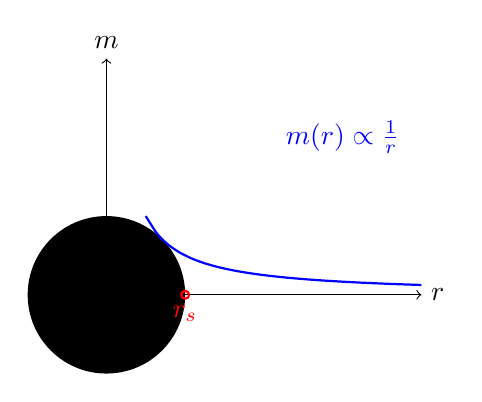
\begin{tikzpicture}
			\fill[black] (0,0) circle (1);
			\draw[->] (0,0) -- (4,0) node[right] {$r$};
			\draw[->] (0,0) -- (0,3) node[above] {$m$};
			\draw[red, thick] (1,0) circle (0.05) node[below] {$r_s$};
			\draw[blue, scale=0.5, domain=1:8, smooth, variable=\x, thick] plot ({\x}, {2/\x});
			\node[blue] at (3,2) {$m(r) \propto \frac{1}{r}$};
		\end{tikzpicture}
		\caption{Black hole in the $T_0$-model: The event horizon ($r_s$) marks the boundary of extreme mass variation, but no singularity at the center.}
	\end{figure}
	
	\section{Effects on the Light Cone}
	The light cone, a central concept in special relativity, defines the causal structure of spacetime, with the speed of light \( c_0 \) marking the boundary between reachable (inside the cone) and unreachable (outside the cone) events. The proposed models significantly alter the interpretation and dynamics of the light cone.
	
	In the standard model, the light cone is determined by the Lorentz transformation, where time dilation (\( t' = \gamma t \)) and length contraction relativistically distort its shape, while rest mass remains constant. The \( T_0 \)-model with absolute time turns this on its head: since \( T_0 \) is constant, time dilation is eliminated, and the causal structure is defined by mass and energy variations (\( m = \gamma m_0 \), \( E = \frac{\hbar}{T_0} \)). The light cone remains geometrically intact, as \( c_0 \) still forms the boundary, but its meaning shifts: instead of temporal relativity, mass determines the reach of events.
	
	\subsection{Reformulation of Causal Structure}
	In the traditional relativistic interpretation, the light cone sets a boundary between causally connected and unconnected events. In the \( T_0 \)-model, however, this causal structure manifests not through time dilation but through mass variation. For an object at high velocity near \( c_0 \), mass increases (\( m = \gamma m_0 \)), while time remains unchanged, leading to a fundamentally different physical interpretation.
	
	This reinterpretation can be formally expressed through the transformation of the light cone operator:
	\begin{equation}
		\mathcal{O}_{\text{std}} = c_0^2 t^2 - |\vec{x}|^2 \quad \rightarrow \quad \mathcal{O}_{T_0} = c_0^2 T_0^2 - |\vec{x}|^2
	\end{equation}
	where \( \mathcal{O} > 0 \) denotes timelike, \( \mathcal{O} = 0 \) lightlike, and \( \mathcal{O} < 0 \) spacelike intervals. In the \( T_0 \)-model, the cone's geometric form persists, but its physical interpretation changes dramatically: the light cone becomes an energy barrier modulated by mass variation.
	
	Concretely, this means an observer at higher velocity does not experience altered time perception but rather an increased effective mass and energy. This leads to a novel conception of causal connection as a function of energy rather than time, with "future" and "past" delineated by mass gradients rather than time intervals. In this formulation, causality is determined not by temporal sequences but by energy states, representing a fundamental reversal of the usual relativistic interpretation.
	
	\subsection{Dynamic Light Cones in the Intrinsic Time Formulation}
	The modified Schrödinger equation with intrinsic time \( T = \frac{\hbar}{m c^2} \) adds another layer of complexity: time evolution within the light cone becomes mass-dependent, leading to a dynamic adjustment of the causal structure. This mass dependence can be formally represented by a modified light cone metric:
	\begin{equation}
		ds^2 = c_0^2 dT^2 - d\vec{x}^2 = c_0^2 \left(\frac{\hbar}{m c^2}\right)^2 dt^2 - d\vec{x}^2 = \frac{\hbar^2}{m^2} dt^2 - d\vec{x}^2
	\end{equation}
	
	For small masses (large \( T \)), the effective time evolution expands, making the light cone appear "wider." This implies that light particles could have a broader causal reach, while heavy particles exhibit a more compressed causal structure. The mathematical consequence is that the light cone is no longer universal for all particles but scales individually:
	\begin{equation}
		\mathcal{O}_T = \frac{\hbar^2}{m^2} t^2 - |\vec{x}|^2
	\end{equation}
	
	This mass-dependent scaling leads to several notable phenomena:
	
	\begin{enumerate}
		\item \textbf{Mass-Dependent Causality}: Particles of different masses experience distinct causal structures. Lighter particles may potentially be causally connected to more events than heavier ones under otherwise identical conditions.
		\item \textbf{Limit Case of Massless Particles}: For photons (\( m = 0 \)), \( T \) would formally become infinite, conflicting with the standard interpretation of the speed of light as a boundary. This necessitates an extension of the model for massless particles, using \( T = \frac{1}{E} = \frac{1}{p} \) for photons, proportional to their wavelength.
		\item \textbf{Quantum Gravitational Effects}: Near the Planck scale, where \( m \approx m_P \), the intrinsic time \( T \approx t_P \), suggesting a fundamental entanglement between causal structure and quantum gravitational effects.
	\end{enumerate}
	
	\subsection{Experimental Consequences}
	The differing interpretations of the light cone in the proposed models lead to potentially testable predictions:
	
	\begin{enumerate}
		\item \textbf{Mass-Dependent Phase Shifts}: In quantum interference experiments, particles of different masses might exhibit distinct phase shifts due to their varying intrinsic times, measurable via high-precision interferometry.
		\item \textbf{Mass-Dependent Coherence Times}: Coherence time in quantum systems could scale with \( T = \frac{\hbar}{m c^2} \), leading to longer coherence times for lighter particles, verifiable in quantum information experiments.
		\item \textbf{Gravitational Lensing Effect}: In strong gravitational fields, light deflection might be modified not only by spacetime curvature but also by mass variation, potentially causing subtle deviations from general relativity.
		\item \textbf{Novel Causality Effects}: In highly relativistic systems, mass-dependent causal structures could lead to unexpected delays or accelerations in signal propagation, measurable through ultra-precise timing.
	\end{enumerate}
	
	\subsection{Theoretical Extensions}
	The reformulation of the light cone opens possibilities for theoretical extensions beyond the standard relativistic interpretation:
	
	\begin{enumerate}
		\item \textbf{Generalized Lorentz Transformation}: A modified Lorentz transformation accounting for mass variation instead of time dilation could be developed:
		\begin{equation}
			m' = \gamma m, \quad E' = \gamma E, \quad T_0' = T_0, \quad x' = \gamma(x - vt), \quad t' = t
		\end{equation}
		This would preserve the light cone's invariance but offer an alternative physical interpretation.
		\item \textbf{Energy-Dependent Metric}: An energy-dependent metric could be formulated, describing the causal structure as a function of local energy gradients rather than spacetime curvature:
		\begin{equation}
			g_{\mu\nu} = \eta_{\mu\nu} + \kappa \frac{\partial E}{\partial x^\mu}\frac{\partial E}{\partial x^\nu}
		\end{equation}
		where \( \kappa \) is a constant determining the strength of this coupling.
		\item \textbf{Extended Causality in Quantum Systems}: The mass-dependent intrinsic time could lead to an expanded definition of causality in quantum systems, where causal order is no longer absolute but relative to the mass of involved particles. This could be formalized by a generalized operator:
		\begin{equation}
			\hat{\mathcal{C}} = \mathcal{T} \exp\left(i\int \frac{dt}{T(m)} \hat{H}(t)\right)
		\end{equation}
		where \( \mathcal{T} \) is the time-ordering operator and \( \hat{H} \) is the Hamiltonian.
	\end{enumerate}
	
	\subsection{Philosophical Reinterpretation of Causality}
	The reformulation of the light cone entails profound philosophical implications for our understanding of causality and time:
	
	In the traditional interpretation of special relativity, the causal structure is secured by the invariance of the light cone under Lorentz transformations, with time dilation emphasizing the relative nature of time. The \( T_0 \)-model reverses this perspective by treating time as absolute and viewing mass as variable. This leads to a fundamental reinterpretation of causality, where energy states, not temporal sequences, determine causal order.
	
	This energy-based causality suggests that what we perceive as temporal order might be an emergent property of more fundamental energy gradients. In this view, the "direction of time" would be dictated not by the flow of time but by the gradient of mass distribution, consistent with the second law of thermodynamics, as energy dissipation provides a natural direction.
	
	The intrinsic time \( T = \frac{\hbar}{m c^2} \) extends this perspective by assigning each particle its own timescale. This results in a relativized causality, where the causal connection between events is not absolute but relative to the mass of the involved particles. This fragmentation of the causal structure challenges the notion of a unified, universal temporal order, suggesting instead a more complex picture where causality is mass-dependent.
	
	Such a reinterpretation could impact our understanding of the arrow of time. While the thermodynamic arrow is given by entropy increase, the causal arrow in this model might be determined by the direction of mass flow or energy dissipation. This would imply that time’s asymmetry is not a fundamental property of spacetime but an emergent feature of energy and mass distribution.
	
	Ultimately, this reinterpretation raises a profound question: Is time a fundamental quantity, or merely an emergent phenomenon arising from more complex interactions between mass and energy? The proposed models suggest the latter, inviting a reconsideration of our understanding of causality, time, and the fundamental structure of reality.
	
\end{document}